% Options for packages loaded elsewhere
\PassOptionsToPackage{unicode}{hyperref}
\PassOptionsToPackage{hyphens}{url}
%
\documentclass[
]{article}
\usepackage{amsmath,amssymb}
\usepackage{iftex}
\ifPDFTeX
  \usepackage[T1]{fontenc}
  \usepackage[utf8]{inputenc}
  \usepackage{textcomp} % provide euro and other symbols
\else % if luatex or xetex
  \usepackage{unicode-math} % this also loads fontspec
  \defaultfontfeatures{Scale=MatchLowercase}
  \defaultfontfeatures[\rmfamily]{Ligatures=TeX,Scale=1}
\fi
\usepackage{lmodern}
\ifPDFTeX\else
  % xetex/luatex font selection
\fi
% Use upquote if available, for straight quotes in verbatim environments
\IfFileExists{upquote.sty}{\usepackage{upquote}}{}
\IfFileExists{microtype.sty}{% use microtype if available
  \usepackage[]{microtype}
  \UseMicrotypeSet[protrusion]{basicmath} % disable protrusion for tt fonts
}{}
\makeatletter
\@ifundefined{KOMAClassName}{% if non-KOMA class
  \IfFileExists{parskip.sty}{%
    \usepackage{parskip}
  }{% else
    \setlength{\parindent}{0pt}
    \setlength{\parskip}{6pt plus 2pt minus 1pt}}
}{% if KOMA class
  \KOMAoptions{parskip=half}}
\makeatother
\usepackage{xcolor}
\usepackage[margin=1in]{geometry}
\usepackage{graphicx}
\makeatletter
\def\maxwidth{\ifdim\Gin@nat@width>\linewidth\linewidth\else\Gin@nat@width\fi}
\def\maxheight{\ifdim\Gin@nat@height>\textheight\textheight\else\Gin@nat@height\fi}
\makeatother
% Scale images if necessary, so that they will not overflow the page
% margins by default, and it is still possible to overwrite the defaults
% using explicit options in \includegraphics[width, height, ...]{}
\setkeys{Gin}{width=\maxwidth,height=\maxheight,keepaspectratio}
% Set default figure placement to htbp
\makeatletter
\def\fps@figure{htbp}
\makeatother
\setlength{\emergencystretch}{3em} % prevent overfull lines
\providecommand{\tightlist}{%
  \setlength{\itemsep}{0pt}\setlength{\parskip}{0pt}}
\setcounter{secnumdepth}{-\maxdimen} % remove section numbering
\ifLuaTeX
  \usepackage{selnolig}  % disable illegal ligatures
\fi
\usepackage{bookmark}
\IfFileExists{xurl.sty}{\usepackage{xurl}}{} % add URL line breaks if available
\urlstyle{same}
\hypersetup{
  pdftitle={Spending start days prediction: Regression Approach},
  pdfauthor={Md Ismail Hossain},
  hidelinks,
  pdfcreator={LaTeX via pandoc}}

\title{Spending start days prediction: Regression Approach}
\author{Md Ismail Hossain}
\date{2025-03-03}

\begin{document}
\maketitle

\newpage

\section{Data Structure:}\label{data-structure}

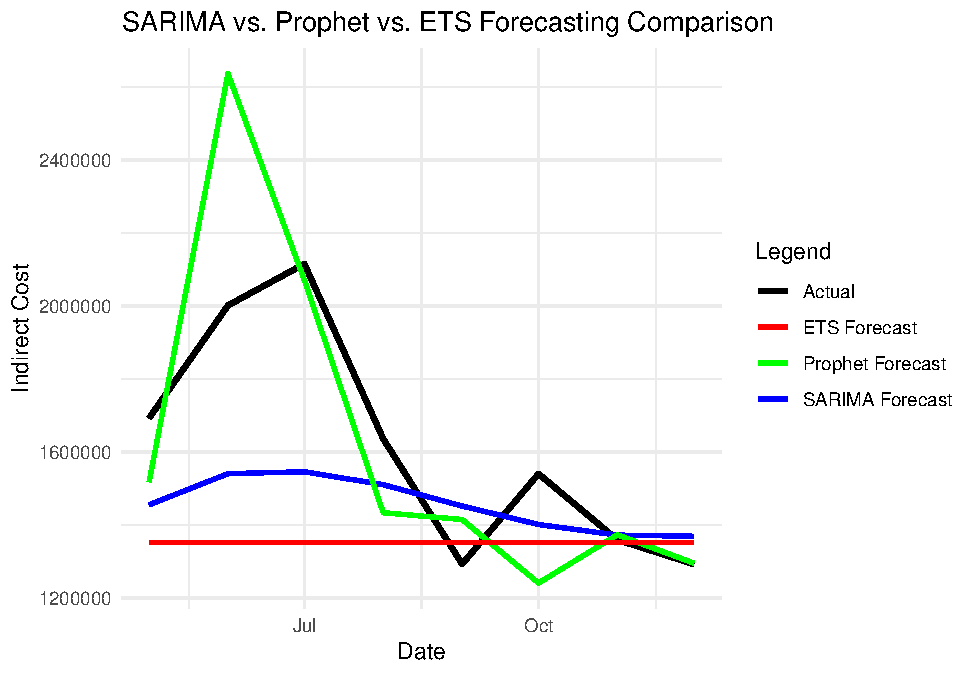
\includegraphics{Regression-Approach_files/figure-latex/unnamed-chunk-3-1.pdf}

\section{Ordinary Least Squares (OLS) Regression
Model}\label{ordinary-least-squares-ols-regression-model}

\begin{verbatim}
## 
## Call:
## lm(formula = Expense_starting_days ~ Number_of_Project_as_Principal_Investigator + 
##     Total_project_person + Project_duration + `Project Funding Amount` + 
##     `Project Funding Type` + `Project Type`, data = project_expenditure_indirect_cost_selected)
## 
## Residuals:
##     Min      1Q  Median      3Q     Max 
## -817.75 -191.81  -10.36  135.42 1044.12 
## 
## Coefficients:
##                                               Estimate Std. Error t value
## (Intercept)                                 -2.658e+02  6.446e+01  -4.124
## Number_of_Project_as_Principal_Investigator  1.891e+00  5.011e-01   3.773
## Total_project_person                         3.229e+01  8.727e+00   3.700
## Project_duration                             3.430e-01  3.084e-02  11.123
## `Project Funding Amount`                    -1.777e-05  5.021e-06  -3.540
## `Project Funding Type`Federal Passthrough    2.034e+02  6.036e+01   3.370
## `Project Funding Type`Internal               1.031e+02  2.973e+02   0.347
## `Project Funding Type`Non-Federal            1.503e+02  5.161e+01   2.912
## `Project Type`UW Grant Cost Share           -1.498e+02  1.094e+02  -1.370
##                                             Pr(>|t|)    
## (Intercept)                                 5.51e-05 ***
## Number_of_Project_as_Principal_Investigator 0.000214 ***
## Total_project_person                        0.000281 ***
## Project_duration                             < 2e-16 ***
## `Project Funding Amount`                    0.000501 ***
## `Project Funding Type`Federal Passthrough   0.000905 ***
## `Project Funding Type`Internal              0.729013    
## `Project Funding Type`Non-Federal           0.004006 ** 
## `Project Type`UW Grant Cost Share           0.172290    
## ---
## Signif. codes:  0 '***' 0.001 '**' 0.01 '*' 0.05 '.' 0.1 ' ' 1
## 
## Residual standard error: 295.3 on 195 degrees of freedom
##   (91 observations deleted due to missingness)
## Multiple R-squared:  0.4898, Adjusted R-squared:  0.4689 
## F-statistic:  23.4 on 8 and 195 DF,  p-value: < 2.2e-16
\end{verbatim}

\section{Poisson Regression for Count
Data}\label{poisson-regression-for-count-data}

\begin{verbatim}
## 
## Call:
## glm(formula = Expense_starting_days ~ Number_of_Project_as_Principal_Investigator + 
##     Total_project_person + Project_duration + `Project Funding Amount` + 
##     `Project Funding Type` + `Project Type`, family = poisson(link = "log"), 
##     data = project_expenditure_indirect_cost_selected)
## 
## Coefficients:
##                                               Estimate Std. Error z value
## (Intercept)                                  4.646e+00  1.116e-02 416.322
## Number_of_Project_as_Principal_Investigator  4.817e-03  8.084e-05  59.591
## Total_project_person                         8.264e-02  1.350e-03  61.235
## Project_duration                             4.371e-04  3.045e-06 143.527
## `Project Funding Amount`                    -3.890e-08  1.327e-09 -29.323
## `Project Funding Type`Federal Passthrough    5.151e-01  1.007e-02  51.167
## `Project Funding Type`Internal               3.489e-01  5.414e-02   6.444
## `Project Funding Type`Non-Federal            3.293e-01  9.216e-03  35.734
## `Project Type`UW Grant Cost Share           -6.289e-01  2.296e-02 -27.391
##                                             Pr(>|z|)    
## (Intercept)                                  < 2e-16 ***
## Number_of_Project_as_Principal_Investigator  < 2e-16 ***
## Total_project_person                         < 2e-16 ***
## Project_duration                             < 2e-16 ***
## `Project Funding Amount`                     < 2e-16 ***
## `Project Funding Type`Federal Passthrough    < 2e-16 ***
## `Project Funding Type`Internal              1.16e-10 ***
## `Project Funding Type`Non-Federal            < 2e-16 ***
## `Project Type`UW Grant Cost Share            < 2e-16 ***
## ---
## Signif. codes:  0 '***' 0.001 '**' 0.01 '*' 0.05 '.' 0.1 ' ' 1
## 
## (Dispersion parameter for poisson family taken to be 1)
## 
##     Null deviance: 66571  on 203  degrees of freedom
## Residual deviance: 37100  on 195  degrees of freedom
##   (91 observations deleted due to missingness)
## AIC: 38562
## 
## Number of Fisher Scoring iterations: 5
\end{verbatim}

\section{Negative Binomial Model}\label{negative-binomial-model}

\begin{verbatim}
## [1] "Mean: 452.816949152542"
\end{verbatim}

\begin{verbatim}
## [1] "Variance: 239579.973181137"
\end{verbatim}

As, Variance \textgreater\textgreater{} Mean (Overdispersion); we are
using Negative Binomial Model.

\begin{verbatim}
## 
## Call:
## glm.nb(formula = Expense_starting_days ~ Number_of_Project_as_Principal_Investigator + 
##     Total_project_person + Project_duration + `Project Funding Amount` + 
##     `Project Funding Type` + `Project Type`, data = project_expenditure_indirect_cost_selected, 
##     init.theta = 1.140417393, link = log)
## 
## Coefficients:
##                                               Estimate Std. Error z value
## (Intercept)                                  4.497e+00  2.048e-01  21.956
## Number_of_Project_as_Principal_Investigator  5.419e-03  1.591e-03   3.405
## Total_project_person                         8.228e-02  2.772e-02   2.969
## Project_duration                             5.364e-04  9.794e-05   5.477
## `Project Funding Amount`                    -4.280e-08  1.602e-08  -2.671
## `Project Funding Type`Federal Passthrough    5.450e-01  1.917e-01   2.843
## `Project Funding Type`Internal               4.017e-01  9.441e-01   0.425
## `Project Funding Type`Non-Federal            3.973e-01  1.640e-01   2.423
## `Project Type`UW Grant Cost Share           -8.692e-01  3.480e-01  -2.498
##                                             Pr(>|z|)    
## (Intercept)                                  < 2e-16 ***
## Number_of_Project_as_Principal_Investigator 0.000661 ***
## Total_project_person                        0.002991 ** 
## Project_duration                            4.32e-08 ***
## `Project Funding Amount`                    0.007570 ** 
## `Project Funding Type`Federal Passthrough   0.004470 ** 
## `Project Funding Type`Internal              0.670520    
## `Project Funding Type`Non-Federal           0.015386 *  
## `Project Type`UW Grant Cost Share           0.012499 *  
## ---
## Signif. codes:  0 '***' 0.001 '**' 0.01 '*' 0.05 '.' 0.1 ' ' 1
## 
## (Dispersion parameter for Negative Binomial(1.1404) family taken to be 1)
## 
##     Null deviance: 312.94  on 203  degrees of freedom
## Residual deviance: 237.04  on 195  degrees of freedom
##   (91 observations deleted due to missingness)
## AIC: 2783.8
## 
## Number of Fisher Scoring iterations: 1
## 
## 
##               Theta:  1.140 
##           Std. Err.:  0.106 
## 
##  2 x log-likelihood:  -2763.801
\end{verbatim}

\begin{verbatim}
##               df       AIC
## ols_model     10  2910.455
## poisson_model  9 38561.620
## negbin_model  10  2783.801
\end{verbatim}

Looks like Negative Binomial is best so far!

\end{document}
